\documentclass[11pt,a4paper]{article}
\usepackage{caption}
\usepackage{listings}
\usepackage{graphicx}
\usepackage{url}

\begin{document}

\title{Final Report \\ \vspace{2mm} {\large Dynamic Visualization of State Transition Systems}}
\author{Alex Aalbertsberg (s1008129)}
\maketitle

\clearpage
\tableofcontents

\clearpage
\section{Introduction}

In the current day and age, model-based software development is a technique that is often used to test the requirements and functionalities of a software system before physically building the system. An example of a type of modelling system that is used in this discipline is a transition system. These are systems that consist of several so-called state diagrams: Diagrams that define the behavior of each individual object, what the object can be (a state) and what actions it can perform to change its state (transitions). If there are many objects present in a software system, it becomes difficult for a user to create a mental picture of the full state of the system.

Therefore, the purpose behind this project was to create a framework for users to create a visual representation of the full transition system while it is simulating the system. This will provide a clear picture of the way in which the system operates.

This document will describe a software system design for an application that is able to dynamically receive information from applications that generate state transitions that occur during a simulation of a transition system. An example of such an application for transition systems is LTS Analyzer (LTSA for short). The visualisation tool will receive the information about these transitions and visually represent them. The intent is to create a cleareer picture of the complete system state for the end user. The system has been set up in a modular way, so that adding additional functionality is not a difficult task. How this modular setup has been established will be described further in the report.

Section 2 will explain the requirements that were set at the start of the project, as well as specify means of testing whether these requirements have been met. Section 3 will explain the design choices that were made during this project, highlight the system that has been built by use of a UML class diagram and provide an overview of the set of commands and respective parameters that the visualisation tool currently supports. Section 4 will provide an overview of the results of the testing methods that were specified in Section 2. Section 5 will draw conclusions about the final product as a whole, as well as provide possible ways to expand upon it. Finally, Section 6 will provide a list of related work and how it relates to this project.

\clearpage
\section{Requirements}

The first stage of the project was to establish proper boundaries for the project. This section lists the requirements that were set for the final product.

The final product of this project should:

\begin{enumerate}
	\item Be able to create an initial visual representation of all objects in a transition system from the simulation tool (e.g. LTSA).
	\item Be able to receive information about state transition steps that are generated during simulation of a transition system by such a simulation tool.
	\item Be able to interpret the received information and translate the abstract syntax that is received to a graphical representation which is also known as the concrete syntax.
	\item Support a preset schema of commands and respective parameters that allows GUI operations to be performed according to what happens in the transition system's simulation.
	\item Update the visual representation (concrete syntax) according to the transition information that has been received.
\end{enumerate}

These requirements were intended to be tested by simulating several scenario's that test the functionality of the command and parameter schema. Examples of these test scenario's are listed below:

\begin{enumerate}
	\item 2 Wolf-cabbage-goat problem scenario's (success and failure)
	\item An elevator with 2 floors
	\item A christmas tree
	\item 2 Dining philosophers problem scenario's  (success and failure)
\end{enumerate}

\clearpage
\section{Technology}

This section will describe the technology that has been used to create the final product. The decisions to utilize the technology listed below were made during the early stages of the project.

\subsection{System Architecture}

Due to the requirement that the final product should be able to receive commands from a multitude of different
transition system tools, the choice was made to keep the visualisation framework separate from the simulation tools. The flowchart below displays the full architecture of how the application operates.

\begin{figure}[ht!]
	\centering
		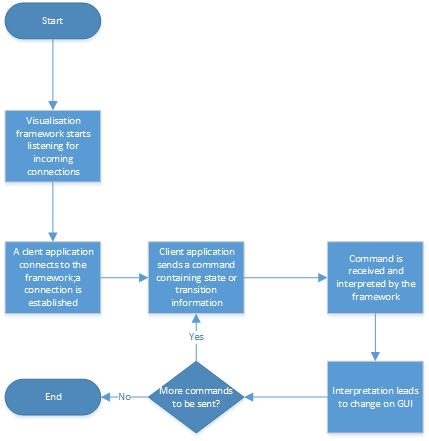
\includegraphics[width=\textwidth]{Flowchart.jpg}
	\caption{Flowchart detailing the process}
\end{figure}

\subsection{Design Choices}

This section will highlight several design choices that were made during the initial phases of the project:

\begin{enumerate}
	\item Paradigm: The method of connection between the simulation tool and the visualisation framework.
	\item Programming Language: What programming language the visualisation framework would be written in.
	\item Data Format: What format should be used to convey information from the simulation tool to the simulation framework.
\end{enumerate}

\subsubsection{Paradigm}

The paradigm that was used for the connection between the visualisation framework and client application is the client-server paradigm. This paradigm is very convenient in this case, as it not only allows a connection to be established between the two communicating applications so that messages may be exchanged, but the two applications do not necessarily have to be present on the system in order to communicate.

\subsubsection{Programming Language}

The programming languages that were available to be chosen from were C\# and Java, based on previous programming experience. Below, a table can be found that lists characteristics for each programming language pertaining to the requirements of the project. The criteria that the table lists are based off of the requirements set for the final product. GUI support is required for being able to show a visual representation of the transition system's state. Networking support was set as a criterion because of the usage of the client-server paradigm, as described in the previous paragraph. Lastly, the multi-platform criterion did not originate from any specific requirement, but was included as a criterion because it would greatly increase usability, as people that wish to use this tool may not all be running the same operating system.
\begin{table}[h]
	\begin{center}
		\begin{tabular}{| c || c | c |}
			\hline
			Criteria & Java & C\# \\ \hline
			GUI Support & Yes, in Java 8 (JavaFX) & Yes \\ \hline
			Networking Support & Yes & Yes \\ \hline
			Multi-OS & Yes & Limited \\ \hline
		\end{tabular}
		\caption{Comparison of Programming Languages}
	\end{center}
\end{table}
\clearpage
As shown in the table, both C\# and Java provide sufficient support when it comes to user interfacing and networking. The deciding factor was the support on multiple platforms. C\# is proprietary to Microsoft .NET, and is therefore limited on platforms other than Microsoft Windows. Based on these criteria, the decision was made to write the application in Java 8 and to use the native library JavaFX for user interfacing. Java has been chosen in order to maintain as much scalability as possible.

\subsubsection{Data Format}

This section will briefly describe the data formats that were available, as well as explain the data format that was chosen based on the criteria listed below. The first criterion for choosing a data format was the amount of overhead that the format generates when sending large amounts of messages. Another criterion was whether the chosen language, Java, provided native support for the data format. The last criterion was how easy it is to parse information. 
\begin{table}[h]
	\begin{center}
		\begin{tabular}{| c || c | c | c |}
			\hline
			Criteria & JSON & CSV & XML \\ \hline
			Overhead & Small & Small & Large \\ \hline
			Language Support & Open-source & None & In-built \\ \hline
			Parseability & Easy & Medium & Easy \\ \hline
		\end{tabular}
		\caption{Comparison of Transport Protocols}
	\end{center}
\end{table}
Based on the above criteria, the decision was made to let communication take place by sending JSON objects over an established TCP connection. XML's large overhead and parsing CSV requiring additional work left JSON to be the best option.
The library that has been used for JSON is the library from www.json.org. Their source code for supporting JSON in Java is freely available on their website.

\subsection{Application Design Specifics}
The application consists of several classes, which have been listed below. This design attempts to maintain a certain level of abstraction, so that expanding upon existing functionality does not require a lot of work.

\begin{enumerate}
\item The Main class. This class initializes the GUI and TCP Server, so that commands may be interpreted and updated on the user interface.
\item The CommandProcessor class. This class deciphers the JSON data sent to the TCP server, interprets and then executes the specified command.
\item The AbsCommand (abstract) class. This class is a framework for the implementation of any command. It only contains a constructor that requires a JSONObject, and a performCommand method that will execute whatever the JSON data tells it to do.
\item All classes that specify a certain command derive from the AbsCommand class.
\item CommandConstants contains a set of static strings that are used to define parameters used by commands.
\item The SocketListener class. This class listens for incoming data on a certain port and sends the received information through to the CommandProcessor.
\item The JSONObject class. This class encapsulates an associative set of objects that can easily be sent over a TCP connection.
\end{enumerate}


\begin{figure}[ht!]
	\centering
		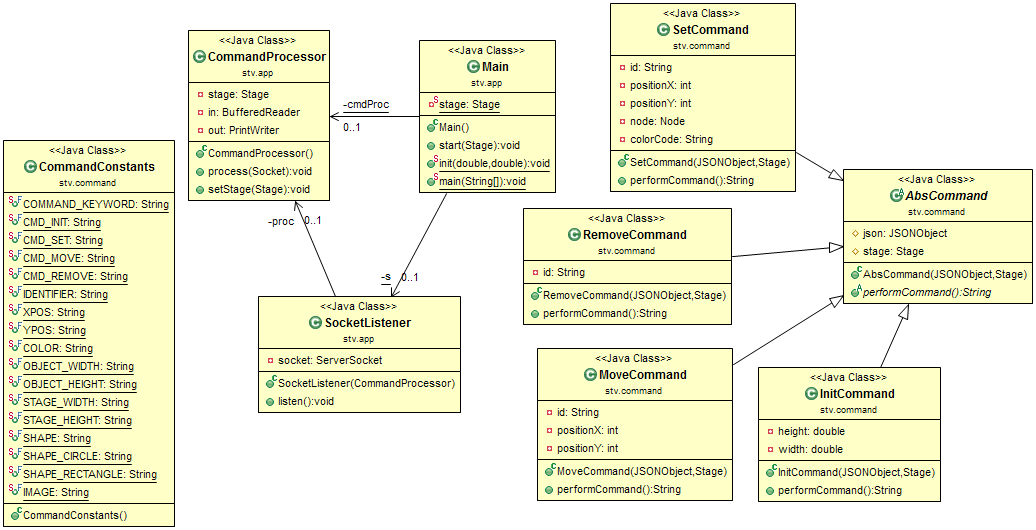
\includegraphics[width=\textwidth]{uml}
	\caption{UML Diagram of the Framework}
\end{figure}

\subsection{Commands and Parameters}

The way in which the client application may communicate with the visualisation framework is by sending commands across the established connection in JSON form. There are four commands available in the final product: Init, Set, Move and Remove. A schema of each command and their respective parameters can be found below. Commands and parameters were created based on the requirements that were to be met by the final product. 

For example, one requirement was that the visualisation framework had to possess the ability to create the initial representation of a transition system. Therefore, the client should be able to send a command to initialize the graphical user interface and create elements that represent the objects in the transition system. For this purpose, the Init and Set commands were created: Init creates the graphical user interface and Set places elements on it. The Move and Remove commands did not originate from a main requirement, but were decided to be a part of the basic GUI operations that were to be supported by the framework.

Extending the framework to support a new command has been kept as simple as possible, as you can see in the UML diagram in the section above. Creating a new command requires a new Command class to be created which will derive from AbsCommand. After this, the performCommand method of the new Command class should be implemented, so that parameters are read from the JSONObject and an action is taken based on what the command should do and the parameters that were received.

At the moment there is very little error-checking in place for these commands. This is a potential and very important improvement that did not take place before the end of this project.

A JSONObject sent across an established connection should contain the command key with a valid command as its value. The commands and corresponding parameters that are currently supported by the application are listed below.


\begin{enumerate}
	\item init. This command allows the user to set initial GUI/application values.
		\begin{enumerate}
			\item GUI width. (``stageWidth'', double)
			\item GUI height. (``stageHeight'', double)
		\end{enumerate}
	\begin{lstlisting}[language=java]
	JSONObject obj = new JSONObject();
	obj.set(``command'', ``init'');
	obj.set(``stageWidth'', 500);
	obj.set(``stageHeight'', 500);
	\end{lstlisting}
	\item set. This command allows the user to create elements on the GUI.
		\begin{enumerate}
			\item Identifier. (``id'', String)
			\item X-axis position. (``posx'', int)
			\item Y-axis position. (``posy'', int)
			\item Color. (``colorCode'', String)
			\item Shape. (``shape'', String (Supported values: ``circle'' or ``rectangle''))
			\item Image. (``image'', Base64 String)
		\end{enumerate}
	\begin{lstlisting}[language=java]
	JSONObject obj = new JSONObject();
	obj.set(``command'',``set'');
	obj.set(``id'',``wolf'');
	obj.set(``posx'', 100);
	obj.set(``posy'', 100);
	obj.set(``image'',``string''[base64]);
	\end{lstlisting}
	\item move. This command allows the user to move existing GUI elements.
		\begin{enumerate}
			\item Identifier of the element to move. (``id'', String)
			\item New X-axis position. (``posx'', int)
			\item New Y-axis position. (``posy'', int)
		\end{enumerate}
	\begin{lstlisting}[language=java]
	JSONObject obj = new JSONObject();
	obj.set(``command'', ``move'');
	obj.set(``id'', ``wolf'');
	obj.set(``posx'', 200);
	obj.set(``posy'', 200);
	\end{lstlisting}
	\item remove. This command allows the user to remove an existing GUI element.
		\begin{enumerate}
			\item Identifier of the element to remove. If the specified identifier does not exist, this command does not have an effect. (``id'', String)
		\end{enumerate}
	\begin{lstlisting}[language=java]
	JSONObject obj = new JSONObject();
	obj.set(``command'', ``remove'');
	obj.set(``id'', ``goat'');
	\end{lstlisting}
\end{enumerate}


\section{Test results}

For the sake of properly testing the final product, a testing method has been defined. We will check the functionalities of the main program with a simulation of the wolf-goat-cabbage problem, as described below. This test will take place with the use of a makeshift client that sends JSON data that corresponds to the wolf-cabbage-goat problem. This data is stored in a plain text file.

\subsection{Wolf-Goat-Cabbage Problem}

This problem deals with the following: A man is standing on the bank of a river with a wolf, a goat and a cabbage. The man wants to cross the river with all three of them. However, his boat will only allow him to take one of the three with him at a time. The other two will have to wait. When the man is not there, the wolf is capable of eating the goat, and the goat is capable of eating the cabbage.

For this problem, both a success and a failure scenario have been created. These scenarios test the functionality of each individual command and operate properly. Of course, the success scenario first places the goat on the other bank, as the wolf and the cabbage share no interaction that would hinder progress. The man could then take either the wolf or the cabbage to the opposite bank (it does not matter which one) and takes the goat back to the first bank. Then, the man will take the wolf or the cabbage (whichever he did not take with him previously). Now, the goat will be the only one left on the first bank, allowing a simple cross to complete the problem. Similarly, the failure scenario moves the cabbage over to the other bank first, causing the wolf to ``eat'' the goat. The goat is then removed from the GUI.

In command form, the success scenario would look like the following:

\begin{enumerate}
	\item Init command: Initialize the GUI at a given width and height.
	\item Set command: Create the element for the wolf. Place the wolf on the left bank of the river.
	\item Set command: Create the element for the goat. Place the goat on the left bank of the river.
	\item Set command: Create the element for the cabbage. Place the cabbage on the left bank of the river
	\item Move command: Move the goat to the right bank.
	\item Move command: Move the cabbage to the right bank.
	\item Move command: Move the goat back to the left bank.
	\item Move command: Move the wolf to the right bank.
	\item Move command: Move the goat to the right bank.
\end{enumerate}

As shown in the enumeration above, the init and set commands can be used quite efficiently to recreate the initial state of the system. After that, the transitions of object states take place. These are represented by the move commands.

Some screenshots of the visualisation process can be found in Appendix A. These screenshots use the success scenario of the wolf-cabbage-goat problem as an example.

\section{Conclusions}

In this section, we will check our final product by the standards of the requirements that were set at the start of the project:

Requirement 1: Be able to create an initial visual representation of a state diagram from the tool that generated said diagram.
Result: The init and set commands provide functionality for an external application to set-up the initial GUI and instantiate objects that require a visual representation.

Requirement 2: Be able to receive information about state transition steps from any state diagram tool.
Result: The application listens for a TCP connection on a certain port. This functionality has been tested by use of a simulated transition system application, where JSON objects are read from a text file and passed to the server as ``simulated states and transitions''.

Requirement 3: Be able to interpret the received information and translate the abstract syntax that is received to a graphical representation which is also known as the concrete syntax.
Result: The application reconstructs the JSON object it receives over the TCP connection and then translates the information contained to operations on the graphical interface.

Requirement 4: Support a preset schema of commands and respective parameters that allows client applications to perform GUI operations according to what happens in the state transitions.
Result: A set of commands and respective parameters has been defined, as well as the commands' respective operations on the graphical user interface.

Requirement 5: Update the visual representation (concrete syntax) according to the transition information that has been received.
Result: Every command in the simulation had the expected effect on the graphical user interface.

All requirements set at the start of the project have been met.

\section{Discussion}

As for future development of this project, there are several things that could be improved upon. First of all, the execution of commands contains very little error-checking at this point in time. This error checking should be built into the implementation of each command, so that the visualisation framework may provide feedback to the end user.

Another improvement that could be made would be to implement new commands: for example, a command that allows modifications to be made to the properties of existing elements. Similarly, there are probably potential improvements to think of for existing commands, such as being able to define a width and height of an element.

The overall result of the project satisfies the requirements and also provides a modular set-up in which adding new functionality is a simple process. Because of this, I feel content with the way the project has gone and the final product.

\section{Related work}

This section will describe the papers that were used as preparation for this project, and how they are related or relevant to the project.

The paper about JTorX and the documentation of TorXviz by A. Belinfante, as well as the papers by Magee et al and van Ham et al were used to create a picture of existing research and development on the subject of the animation of transition systems, as well as to potentially provide useful insight in how this project should be developed.

The paper by Diethelm et al was examined to check whether it was viable to use their framework named WhiteSocks to implement the user interface of the visualisation framework. However, after coming into contact with one of the developers of WhiteSocks, it was learned that development of the framework had been discontinued. The developers had started using JavaFX instead.

\clearpage
\section{Appendices}

\subsection{Appendix A: Simulation Screenshots}

\begin{figure}[ht!]
	\centering
		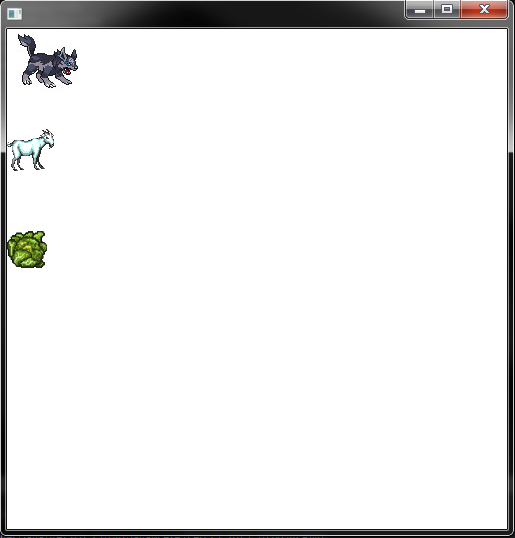
\includegraphics[width=\textwidth]{1}
	\caption{Initial state}
\end{figure}

\begin{figure}[ht!]
	\centering
		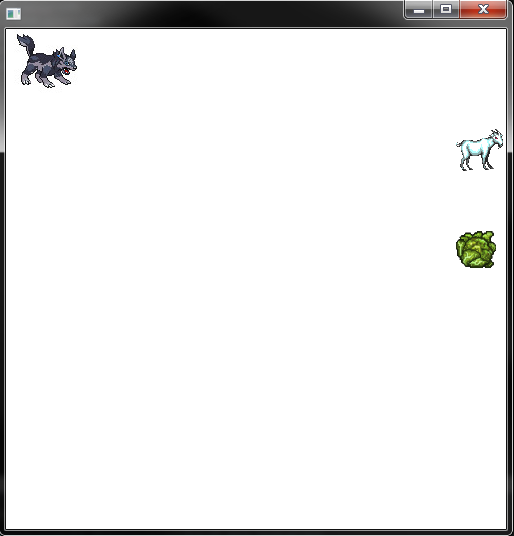
\includegraphics[width=\textwidth]{2}
	\caption{Mid-execution}
\end{figure}

\begin{figure}[ht!]
	\centering
		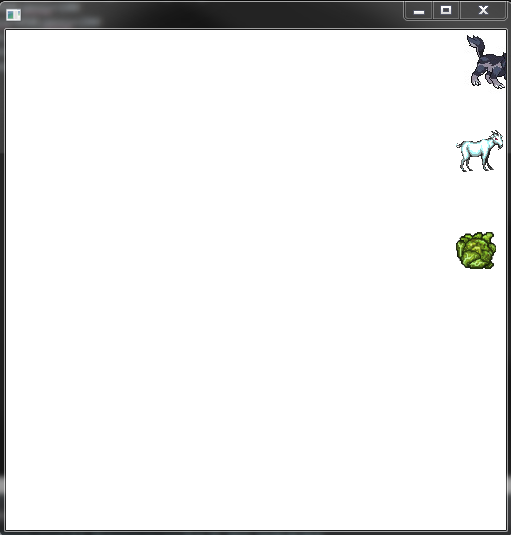
\includegraphics[width=\textwidth]{3}
	\caption{Final state}
\end{figure}

\clearpage

\bibliography{bibliography}
\bibliographystyle{plain}

\nocite{*}

\end{document}